\scanpage{62}
% E: text|printed top seven lines|HASP373 STARTED
\texttt{\unsure{\$HASP373} STARTED - INIT 2 - CLASS 1 - SYS E333}\par
\texttt{IEF236I ALLOC. FOR CRAY2}\par
\texttt{IEF142I CRAY2 - STEP WAS EXECUTED - COND CODE 0000}\par
\texttt{IEF373I STEP /\qquad / START 82229.0906}\par
\texttt{IEF374I STEP /\qquad / STOP 82229.0906 CPU 0MIN 00.01SEC SRB 0MIN 00.00SEC VIRT 8K SYS 200K}\par
\texttt{IEF375I JOB /CRAY2\qquad / START 82229.0906}\par
\texttt{IEF376I JOB /CRAY2\qquad / STOP 82229.0906 CPU 0MIN 00.01SEC SRB 0MIN 00.00SEC}
% E: diagram|upper left handwritten first line|F=FD to FDprime=Fprime
\diagram{\begin{tikzcd}
F=F_D\arrow[r] & F_{D'}=F'
\end{tikzcd}}
% E: diagram|left three rows of orientation objects|omega FD omega F omega D
\diagram{\begin{tikzcd}[row sep=large,column sep=huge]
\omega(F_D)\arrow[r,"\alpha\ \text{transport parallèle}","\unsure{\text{c.-à-d. via les }\operatorname{Pol}(D)}"']\arrow[d,phantom,"{\rotatebox{90}{$\simeq$}}" description] & \omega(F_{D'})\arrow[d,phantom,"{\rotatebox{90}{$\simeq$}}" description]\\
\omega(\unsure{F|\overline F})\arrow[r,"\beta\ \text{transport de}","\text{l'orientation sur }X"']\arrow[d,phantom,"{\rotatebox{90}{$\simeq$}}" description] & \omega(F')\arrow[d,phantom,"{\rotatebox{90}{$\simeq$}}" description]\\
\omega(D)\arrow[r,"\alpha'\ \text{transport parallèle}"] & \omega(D')
\end{tikzcd}}
% E: drawing|upper middle pencil sketch|two nearly tangent loops
\figure{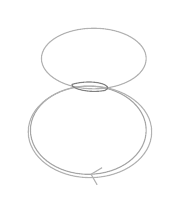
\begin{tikzpicture}[scale=.7]
\draw[gray!60] (.1,1.3) ellipse (.95 and .55);
\draw[gray!70] (0,0) ellipse (1.05 and .8);
\draw[gray!60] (.03,-.03) ellipse (1.12 and .83);
\draw[gray] (-.3,.83)..controls (.1,.95) and (.5,.8)..(.3,.72)..controls (0,.67) and (-.3,.75)..(-.3,.83);
\draw[gray!60] (.05,-.8)--(.25,-.68) (.05,-.8)--(.16,-.99);
\end{tikzpicture}}
% E: drawing|right middle|sigmoid line crossed by three verticals
\figure{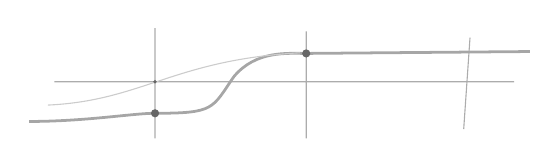
\begin{tikzpicture}[scale=.8]
\draw[gray!65] (-3,0)--(4.3,0) (-1.4,-.9)--(-1.4,.85) (1,-.9)--(1,.8) (3.5,-.75)--(3.6,.7);
\draw[gray!70,line width=1pt] (-3.4,-.63)..controls (-2.5,-.63) and (-1.75,-.5)..(-1.4,-.5)..controls (-.45,-.5) and (-.5,-.43)..(-.15,.08)..controls (.2,.5) and (.7,.45)..(1,.45)--(4.55,.48);
\draw[gray!40] (-3.1,-.37)..controls (-1.6,-.3) and (-1.1,.35)..(.9,.46);
\fill[gray!80!black] (-1.4,-.5) circle(.065) (1,.45) circle(.065) (-1.4,0) circle(.03);
\end{tikzpicture}}
% E: display|middle lower relation between alpha and beta|alpha=alpha prime
\[\alpha=\alpha'\qquad\beta=\alpha,\alpha'\quad\text{ssi. nb d'opérations }\inserted{N}\text{ est pair}\]
% E: display|lower example line|ex F=FDprime
\[\text{ex }F=F_{D'},\quad\alpha=\alpha'=-1\qquad\text{alors }\beta=-1\quad\text{ssi }\deleted{\unsure{nb}}\ N\text{ pair}\]
% E: text|lower left unfinished conclusion|donc
 donc
\mspage{61}
